\chapter{Разработка окон управления}
\label{cha:ch_3}
При создании окон управления не были использованы ни синглтон заготовки, ни написанный DI контейнер ввиду особенностей распределения времени выполнения  у \textit{Unity} -- пространство имен, взаимодействующее с классами, которые регламентируют внешний вид и поведение пользовательских окон, изолировано от других пространств, что делает невозможным использование DI и других вспомогательных структур. 

\section{Создание окна управления записью и проигрыванием}
Данное окно (см. рис. \ref{recorderUI}) состоит из трёх секций: указание текущей реализации проигрывателя, состояние проигрывателя и элементы управления проигрыванием и записью.

\begin{figure}[h]
	\centering
	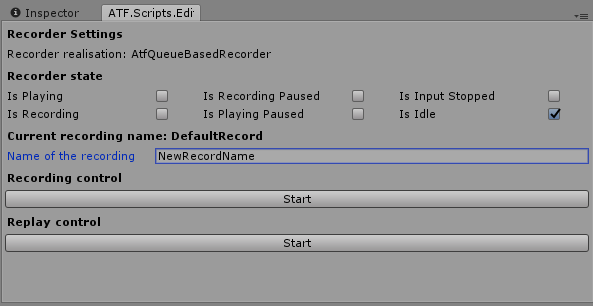
\includegraphics[width=0.7\linewidth]{recorder.PNG}
	\caption{Editor UI для проигрывателя}
	\label{recorderUI}
\end{figure}

В процесс управления записью входит:
\begin{itemize}
	\item
	просмотр текущего состояния проигрывателя по чекбоксам состояния на рис.\ref{recorderUI};
	\item
	определение имени записи, которую нужно проиграть или под которое нужно записать поток действий;
	\item
	непосредственно сами кнопки управления записью -- Start, Stop, Play, Continue;
	\item
	аналогичные кнопки управления проигрыванием -- Start, Stop, Play, Continue.
\end{itemize}
Для того чтобы проиграть выбранную запись, необходимо сначала вписать нужное имя в поле \textit{Name of the recording} или же просто щёлкнуть правой кнопкой мыши по записи в активной зоне окна управления хранилищем.

\section{Создание окна управления хранилища действий}
Окно управления хранилищем (см. рис. \ref{storageUI}) также состоит из трёх секций -- информация о реализации, секции управления сохранением и загрузкой, а также зоны иллюстрации текущего состояния хранилища.

\begin{figure}[h]
	\centering
	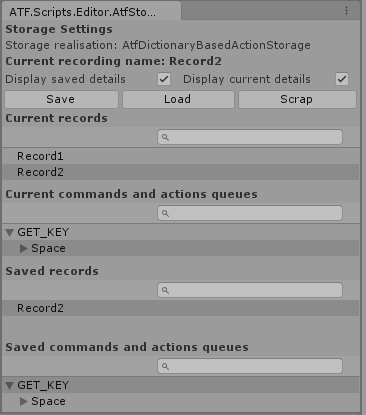
\includegraphics[width=0.7\linewidth]{storage.PNG}
	\caption{Editor UI для хранилища действий}
	\label{storageUI}
\end{figure}

В процесс управления хранилищем входит:
\begin{itemize}
	\item
	просмотр текущей записи хранилища;
	\item
	определение имени записи, которую нужно загрузить или сохранить; 
	\item
	непосредственно сами кнопки управления сохранением -- Save, Load, Scrap (удалить);
	\item
	загрузка в активную зону записей из реестра (Окна: Current records, Current commands and actions queues).
\end{itemize}
Зоны иллюстрации хранилища делятся на активную и пассивную. Активная зона хранит в себе те записи, которые находятся сейчас непосредственно в оперативной памяти, пассивная же зона хранит в себе записи, которые были сохранены на внешнем накопителе или реестре.
